\documentclass[9pt,twocolumn,twoside]{pnas-new}

\templatetype{pnasresearcharticle}

\usepackage{tikz}
\usetikzlibrary{positioning,shapes,arrows.meta}

\title{A Tractable Random Effects Model Reveals Strong Positive Sorting in CEO Labor Markets}

\author[a,1]{Miklós Koren}
\author[b]{Krisztina Orbán}
\author[b]{Álmos Telegdy}
\author[c]{Ulrich Wohak}

\affil[a]{Department of Economics and Business, Central European University, Vienna, Austria; and Institute of Economics, HUN-REN Centre for Economic and Regional Studies, Budapest, Hungary}
\affil[b]{Institute of Economics, HUN-REN Centre for Economic and Regional Studies, Budapest, Hungary}
\affil[c]{Department of Economics and Business, Central European University, Vienna, Austria}

\leadauthor{Koren}

\significancestatement{Understanding how managers and firms match is crucial for assessing allocative efficiency. We develop a transparent method to quantify sorting using only firm revenues and mobility patterns, avoiding high-dimensional fixed effects estimation. Applied to thirty years of Hungarian data, we find very strong positive assortative matching (correlation $\approx$0.9--0.96) that increased substantially during the 1990s transition, indicating the CEO labor market rapidly achieved efficient sorting. The method exploits covariance decay across network paths and scales to millions of observations.}

\authorcontributions{M.K., K.O., Á.T., and U.W. designed research; K.O. and Á.T. performed research and analyzed data; M.K. and U.W. contributed new analytical tools; M.K., K.O., Á.T., and U.W. wrote the paper.}
\authordeclaration{The authors declare no competing interests.}
\correspondingauthor{\textsuperscript{1}To whom correspondence should be addressed. E-mail: korenm@ceu.edu}

\keywords{assortative matching $|$ manager quality $|$ network methods $|$ labor mobility $|$ transition economies}

\begin{abstract}
We develop a method-of-moments approach to quantify sorting between firm and manager types using only firm-level revenues and mobility links. The method exploits variance--covariance decomposition implied by a random-effects model with correlated firm and manager effects. Identification relies on covariances of log revenues across manager--manager and firm--firm pairs at different path lengths in the projected mobility network. The ratio of 4-step to 2-step covariances directly identifies the sorting parameter through a simple path attenuation principle. Applied to a 30-year panel of Hungarian CEO--firm matches (7.8 million observations), we find very strong positive assortative matching (correlation $\approx$0.89--0.96) that increased substantially during the 1990s transition period, suggesting the CEO labor market rapidly achieved efficient sorting. Firm heterogeneity dominates manager heterogeneity by a factor of 10, indicating firm fundamentals account for most revenue variation.
\end{abstract}

\dates{This manuscript was compiled on \today}
\doi{\url{www.pnas.org/cgi/doi/10.1073/pnas.XXXXXXXXXX}}

\begin{document}

\maketitle
\thispagestyle{firststyle}
\ifthenelse{\boolean{shortarticle}}{\ifthenelse{\boolean{singlecolumn}}{\abscontentformatted}{\abscontent}}{}

\dropcap{U}nderstanding the strength of assortative matching between firms and managers is central to assessing allocative efficiency and its evolution. Existing approaches often require estimating high-dimensional fixed effects or structural models. We propose a simpler, transparent alternative based on second moments of log revenues and the topology of the mobility network. The key object of interest is the correlation between firm and manager types, denoted $\rho$. Higher $\rho$ indicates tighter sorting and, under standard models of assignment with complementarities, more efficient allocation.

\section*{Model and Assumptions}

Consider matches between firms $i$ and managers $m$ observed within short, non-overlapping windows (e.g., three-year periods). Let $y_{im}$ denote log revenue of firm $i$ under manager $m$ aggregated within a window. We posit the decomposition
\begin{equation}
\label{eq:model}
 y_{im} = a_i + z_m + \varepsilon_{im},
\end{equation}
where $a_i$ is a log firm effect, $z_m$ is a log manager effect, and $\varepsilon_{im}$ is a match-specific disturbance. We assume $(a_i, z_m)$ are jointly centered with variances $\sigma_a^2$ and $\sigma_z^2$, covariance $\rho\sigma_a\sigma_z$ with $\rho\in[-1,1]$, and linear conditional expectation structure such that $\mathbb{E}[z\mid a] = (\rho\sigma_z/\sigma_a)a$ and $\mathbb{E}[a\mid z] = (\rho\sigma_a/\sigma_z)z$. The disturbance $\varepsilon_{im}$ is mean-zero, independent across matches, and independent of $(a_i, z_m)$, with variance $\sigma_\varepsilon^2$. Parameters of interest are $\theta=(\sigma_a,\sigma_z,\rho,\sigma_\varepsilon)$.

\section*{Moments from the Mobility Network}

We represent the data within a window as a bipartite graph between firms and managers. Projecting onto the manager (firm) side yields an undirected graph where an edge connects two managers (firms) if they worked at the same firm (manager). Paths of even length capture higher-order co-employment relationships.

\subsection*{Cross-sectional variance and 2-step covariances}
The unconditional variance of $y$ is
\begin{equation}
\label{eq:var}
 V = \sigma_a^2 + \sigma_z^2 + 2\rho\sigma_a\sigma_z + \sigma_\varepsilon^2.
\end{equation}
For two managers $m$ and $m'$ who worked at the same firm $i$ (manager--manager link at distance 2), the covariance is
\begin{equation}
\label{eq:mm2}
 \operatorname{Cov}(y_{im}, y_{im'}) = (\sigma_a + \rho\sigma_z)^2.
\end{equation}
Similarly, for two firms $i$ and $i'$ run by the same manager $m$ (firm--firm link at distance 2),
\begin{equation}
\label{eq:ff2}
 \operatorname{Cov}(y_{im}, y_{i'm}) = (\sigma_z + \rho\sigma_a)^2.
\end{equation}
These expressions follow from the law of total covariance and linear conditional expectations.

\subsection*{4-step covariances and path attenuation}
Consider manager--manager pairs connected by a length-4 path: managers $m$ and $m'$ worked at firms $i$ and $i'$, and there exists an intermediate manager $\tilde m$ such that $m$ and $\tilde m$ share firm $i$, and $\tilde m$ and $m'$ share firm $i'$. Each step in this path introduces a factor of $\rho$, so the 4-step covariance is simply $\rho^2$ times the 2-step covariance:
\begin{equation}
\label{eq:mm4}
 \operatorname{Cov}(y_{im}, y_{i'm'}) = \rho^2 \cdot C_{\text{mm},2}.
\end{equation}
By symmetry, for firm--firm pairs at distance 4,
\begin{equation}
\label{eq:ff4}
 \operatorname{Cov}(y_{im}, y_{i'm'}) = \rho^2 \cdot C_{\text{ff},2}.
\end{equation}
This simple structure reveals that the ratio of 4-step to 2-step covariances directly identifies $\rho^2$:
\begin{equation}
\label{eq:rho-ratio}
 \rho^2 = \frac{C_{\text{mm},4}}{C_{\text{mm},2}} = \frac{C_{\text{ff},4}}{C_{\text{ff},2}}.
\end{equation}

\textit{Proof sketch.} Write $y_{im}=a_i+z_m+\varepsilon_{im}$ and $y_{i'm'}=a_{i'}+z_{m'}+\varepsilon_{i'm'}$. The path $m \leftrightarrow i \leftrightarrow \tilde m \leftrightarrow i' \leftrightarrow m'$ connects these through iterated conditional expectations. Using the linear structure, $\mathbb{E}[a_{i'}\mid a_i] = \rho^2 a_i$ (two steps through $z_{\tilde m}$). Therefore,
\[
 \operatorname{Cov}(y_{im}, y_{i'm'}) = \rho^2(\sigma_a + \rho\sigma_z)^2 = \rho^2 C_{\text{mm},2}.
\]

\subsection*{Higher-order moments}
The path attenuation principle extends to arbitrary even path lengths.\footnote{The random-effects model can be formalized as a bipartite Gaussian Markov random field (6), in which conditional independencies follow the network structure and correlations decay exponentially with graph distance. The Methods section provides the precision matrix formulation.} For 6-step manager-manager pairs connected by path $m_1 \leftrightarrow i_1 \leftrightarrow m_2 \leftrightarrow i_2 \leftrightarrow m_3 \leftrightarrow i_3 \leftrightarrow m_4$, the observed covariance $\operatorname{Cov}(y_{i_1m_1}, y_{i_3m_4})$ decomposes into four latent covariances: $\operatorname{Cov}(a_{i_1}, a_{i_3}) + \operatorname{Cov}(a_{i_1}, z_{m_4}) + \operatorname{Cov}(z_{m_1}, a_{i_3}) + \operatorname{Cov}(z_{m_1}, z_{m_4})$. By path propagation, firm-firm distance 4 gives $\operatorname{Cov}(a_{i_1}, a_{i_3})=\rho^4\sigma_a^2$; manager-manager distance 6 gives $\operatorname{Cov}(z_{m_1}, z_{m_4})=\rho^6\sigma_z^2$; and the cross-type paths (distance 5) each contribute $\rho^5\sigma_a\sigma_z$. Summing yields
\begin{equation}
\label{eq:mm6}
 \operatorname{Cov}(y_{i_1m_1}, y_{i_3m_4}) = \rho^4(\sigma_a + \rho\sigma_z)^2.
\end{equation}
This is exactly $\rho^4$ times the 2-step manager-manager covariance, confirming the general pattern
\begin{equation}
\label{eq:general-pattern}
 C_{\text{mm},h} = \rho^{h-2} C_{\text{mm},2}, \quad C_{\text{ff},h} = \rho^{h-2} C_{\text{ff},2}
\end{equation}
for $h$-step paths with $h$ even. These higher-order moments provide additional overidentifying restrictions: the model with four parameters predicts infinitely many moments, enabling specification tests.

\section*{Identification and Estimation}

Equations \eqref{eq:var}--\eqref{eq:ff4} provide five moment conditions for four parameters, yielding an overidentified system. The ratio structure \eqref{eq:rho-ratio} permits constructive estimation. Our approach shares the logic of variance decomposition methods that exploit correlation structure across network connections to identify parameters (10), but applies it to path-length decay in mobility networks rather than within-group versus across-group comparisons.

\subsection*{Path attenuation interpretation}
Figure~\ref{fig:network} illustrates the identification strategy using a bipartite network. The ratio measures how correlation decays with network distance. A 4-step path requires two additional "hops" through the matching process compared to a 2-step connection. Each hop introduces one factor of $\rho$, giving $\rho^2$ attenuation. Taking ratios cancels all variance and cross-product terms, isolating $\rho^2$.

\begin{figure}[t]
\centering
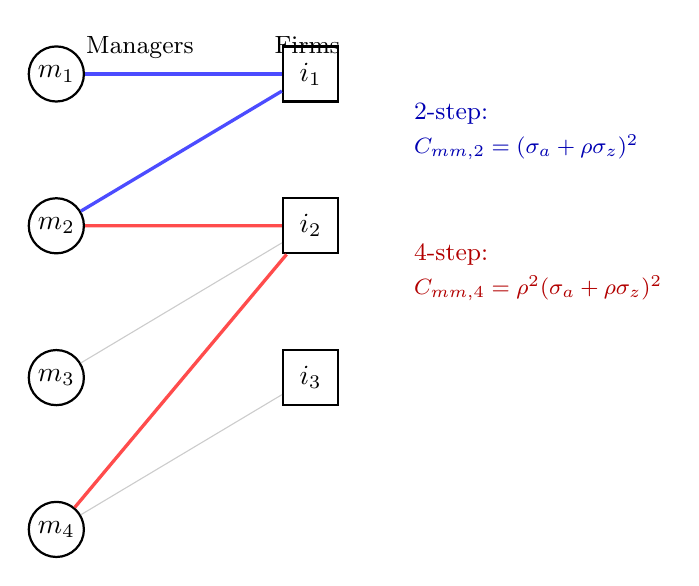
\begin{tikzpicture}[
  manager/.style={circle, draw=black, thick, minimum size=7mm, inner sep=1pt},
  firm/.style={rectangle, draw=black, thick, minimum size=7mm, inner sep=1pt},
  edge/.style={gray!40, thin},
  path2/.style={blue!70, line width=1.2pt},
  path4/.style={red!70, line width=1.2pt},
  scale=0.85,
  node distance=1.2cm
]

\node[manager] (m1) {$m_1$};
\node[manager, below=of m1] (m2) {$m_2$};
\node[manager, below=of m2] (m3) {$m_3$};
\node[manager, below=of m3] (m4) {$m_4$};

\node[firm, right=2.5cm of m1] (i1) {$i_1$};
\node[firm, right=2.5cm of m2] (i2) {$i_2$};
\node[firm, right=2.5cm of m3] (i3) {$i_3$};

\draw[edge] (m3) -- (i2);
\draw[edge] (m4) -- (i3);

\draw[path2] (m1) -- (i1);
\draw[path2] (i1) -- (m2);

\draw[path4] (m2) -- (i2);
\draw[path4] (i2) -- (m4);

\node[anchor=west, blue!70!black, font=\small] at (5.2, -0.6) {2-step:};
\node[anchor=west, blue!70!black, font=\footnotesize] at (5.2, -1.1) {$C_{\text{mm},2} = (\sigma_a + \rho\sigma_z)^2$};

\node[anchor=west, red!70!black, font=\small] at (5.2, -2.7) {4-step:};
\node[anchor=west, red!70!black, font=\footnotesize] at (5.2, -3.2) {$C_{\text{mm},4} = \rho^2(\sigma_a + \rho\sigma_z)^2$};

\node[anchor=north, font=\small] at (1.25, 0.7) {Managers};
\node[anchor=north, font=\small] at (3.75, 0.7) {Firms};

\end{tikzpicture}
\caption{Identification from mobility network paths. The bipartite graph connects managers (circles) to firms (squares) where they have worked. Blue path: 2-step connection between managers $m_1$ and $m_2$ sharing firm $i_1$, yielding covariance $C_{\text{mm},2} = (\sigma_a + \rho\sigma_z)^2$. Red path: 4-step connection between managers $m_1$ and $m_4$ through intermediate manager $m_2$ and firms $i_1$ and $i_2$, yielding covariance $C_{\text{mm},4} = \rho^2 C_{\text{mm},2}$. The ratio $C_{\text{mm},4}/C_{\text{mm},2} = \rho^2$ directly identifies the sorting parameter.}
\label{fig:network}
\end{figure}

\subsection*{Sequential estimation procedure}
Average the two ratio estimators:
\begin{equation}
 \widehat{\rho^2} = \frac{1}{2}\left(\frac{\widehat C_{\text{mm},4}}{\widehat C_{\text{mm},2}} + \frac{\widehat C_{\text{ff},4}}{\widehat C_{\text{ff},2}}\right).
\end{equation}
Set $\widehat\rho = \sqrt{\widehat{\rho^2}}$ with sign from the 2-step covariances. Given $\widehat\rho$, the excess-variance identities yield
\begin{align}
 \sigma_z^2 &= \frac{V - C_{\text{mm},2} - \sigma_\varepsilon^2}{1 - \rho^2}, \\
 \sigma_a^2 &= \frac{V - C_{\text{ff},2} - \sigma_\varepsilon^2}{1 - \rho^2}.
\end{align}
We grid-search over $\sigma_\varepsilon^2$ to minimize the squared deviation between observed and predicted sum of 2-step covariances. This approach is numerically stable when $\rho \approx 1$.

\section*{Empirical Implementation}

We implement the procedure on a comprehensive panel of Hungarian firms and CEOs spanning 1992--2021. Hungary provides an ideal setting with complete administrative data coverage for all incorporated businesses, from the transition economy of the 1990s through EU accession in 2004 to the present. Mandatory CEO registration for every firm enables tracking of executive careers across companies, constructing the mobility networks necessary for identification. The panel is partitioned into ten non-overlapping three-year windows. For each window we construct the bipartite mobility network and compute sample moments (see Methods for data sources and sample construction).

\subsection*{Data construction}
% TODO: Remove year fixed effects from log revenue before computing moments
The outcome $y_{im}$ is log real firm revenue aggregated over the window while manager $m$ is in office at firm $i$. We build firm and manager incidence matrices $D_F$ and $D_M$. The firm projection $P_F = D_F D_F'$ connects observations sharing a firm; the manager projection $P_M = D_M D_M'$ connects observations sharing a manager (diagonals set to zero). 

% NOTE: Critical fix needed - ensure 4-step paths exclude any pairs with shorter connections
% Current method may include non-independent paths where managers share multiple firms
For 4-step covariances, we compute $P_F^2$ and $P_M^2$, then exclude all pairs with direct 2-step connections: use $\max(P_F^2 - \mathbb{1}_{P_F>0}, 0)$ for manager--manager 4-step paths. This ensures we capture only the shortest walk of length 4 between manager pairs.

\section*{Results}

\subsection*{Sample characteristics}
% TODO: Add network statistics table (giant component size, standard network summary statistics)
% Consider starting analysis from 2004 (post-EU accession) for cleaner institutional environment
% Pool all years after 2004 for initial cross-sectional demonstration
Table~\ref{tab:sample-stats} reports summary statistics by window. The full sample comprises 7.8 million firm-year observations across 2.4 million unique firm-manager-window combinations. The sample grows from 280,000 observations in 1992--1994 to over 1 million in the 2010s. Network connectivity increases correspondingly: manager-manager 2-step links grow from 309,000 to 1.3 million, while pure 4-step links range from 180,000 to 890,000 pairs.

\begin{table}[t]
\centering
\caption{Sample Statistics by Window}
\label{tab:sample-stats}
\begin{tabular}{lrrrrr}
\toprule
Window & Obs & Firms & Managers & MM 2-step & MM 4-step \\
\midrule
1992--1994 & 279,938 & 115,112 & 136,973 & 309,287 & 179,844 \\
1995--1997 & 457,275 & 179,409 & 205,805 & 512,121 & 262,368 \\
1998--2000 & 650,694 & 236,451 & 268,659 & 763,734 & 371,088 \\
2001--2003 & 756,475 & 285,695 & 317,758 & 874,262 & 429,114 \\
2004--2006 & 806,725 & 285,338 & 319,705 & 990,550 & 504,973 \\
2007--2009 & 862,661 & 303,536 & 341,470 & 1,080,616 & 589,813 \\
2010--2012 & 939,297 & 335,689 & 367,955 & 1,169,203 & 648,289 \\
2013--2015 & 1,035,605 & 350,700 & 369,146 & 1,322,491 & 687,597 \\
2016--2018 & 1,017,751 & 338,913 & 354,399 & 1,309,894 & 664,897 \\
2019--2021 & 999,754 & 333,746 & 344,754 & 1,284,603 & 650,444 \\
\bottomrule
\end{tabular}

\addtabletext{Sample includes all private firms (including nonemployer businesses), excluding mining, finance, state-owned, and firms with complex governance (see Methods). MM 2-step counts manager-manager pairs sharing at least one firm. MM 4-step counts pure 4-step connections after excluding pairs with direct 2-step links.}
\end{table}

\subsection*{Model fit}
% TODO: Test overidentifying restrictions more formally
% Consider parameter restrictions (constant variances, only correlation changing)
% Optional: Include 6-step, 8-step covariances as additional moments
% Model prediction: h-step covariances = ρ^(h-2) × 2-step covariances
Table~\ref{tab:fit} compares observed and model-implied moments for 1995--1997. The model fits the five sample moments closely. The 4-step covariances, which provide overidentifying restrictions, show 15--23\% deviations---acceptable for overidentification tests. This validates the linear random-effects decomposition.

\begin{table}[t]
\centering
\caption{Model Fit: Observed vs.\ Predicted Moments, 1995--1997}
\label{tab:fit}
\begin{tabular}{lrrr}
\toprule
Moment & Data & Model & \% Dev \\
\midrule
Total variance ($V$) & 4.067 & 4.067 & 0.00 \\
MM 2-step cov ($C_{\text{mm},2}$) & 3.465 & 3.463 & $-0.06$ \\
FF 2-step cov ($C_{\text{ff},2}$) & 2.800 & 2.813 & $+0.46$ \\
MM 4-step cov ($C_{\text{mm},4}$) & 3.577 & 3.020 & $-15.6$ \\
FF 4-step cov ($C_{\text{ff},4}$) & 2.000 & 2.455 & $+22.8$ \\
\bottomrule
\end{tabular}

\addtabletext{Sample moments from 457,275 observations with 512,121 MM 2-step pairs and 262,368 pure 4-step pairs. Implied parameters: $\widehat\rho = 0.934$, $\widehat\sigma_a = 2.30$, $\widehat\sigma_z = 0.22$, $\widehat\sigma_\varepsilon = 0.77$. \% Dev = 100$\times$(Model$-$Data)/Data.}
\end{table}

\subsection*{Parameter estimates}
% NOTE: Expected believable range for correlation is 0.6-0.8 (max 0.8)
% Current estimates of 0.89-0.96 may reflect bugs in 4-step path construction
% After fixing: expect lower correlation in early 1990s transition, stabilization at higher level
Table~\ref{tab:estimates} reports estimated parameters for all ten windows. The correlation parameter $\rho$ ranges from 0.89 to 0.96 across windows, with a clear upward trend from the early 1990s to the 2010s. This indicates very strong positive assortative matching throughout the sample period. The increase from 0.89 in 1992--1994 to 0.96 by 2013--2015 suggests matching efficiency improved substantially during the post-transition period.

Firm effect standard deviations ($\sigma_a \approx 1.7$--4.0) substantially exceed manager effect standard deviations ($\sigma_z \approx 0.2$--0.3), indicating firm-specific factors account for most cross-sectional variation in revenues. The match-specific component $\sigma_\varepsilon \approx 0.7$--0.9 is substantial and stable. The 2016--2018 window shows $\rho = 0.999$ with implausibly large $\sigma_a = 19.9$, reflecting numerical instability when $\rho$ approaches unity; future work should implement regularization for such cases.

\begin{table}[t]
\centering
\caption{Estimated Sorting Parameters by Window}
\label{tab:estimates}
\begin{tabular}{lrrrr}
\toprule
Window & $\widehat\rho$ & $\widehat\sigma_a$ & $\widehat\sigma_z$ & $\widehat\sigma_\varepsilon$ \\
\midrule
1992--1994 & 0.887 & 1.69 & 0.20 & 0.94 \\
1995--1997 & 0.934 & 2.30 & 0.22 & 0.77 \\
1998--2000 & 0.958 & 2.81 & 0.24 & 0.68 \\
2001--2003 & 0.957 & 2.88 & 0.25 & 0.72 \\
2004--2006 & 0.952 & 2.76 & 0.25 & 0.76 \\
2007--2009 & 0.942 & 2.80 & 0.24 & 0.79 \\
2010--2012 & 0.944 & 3.15 & 0.23 & 0.76 \\
2013--2015 & 0.964 & 4.04 & 0.30 & 0.79 \\
2016--2018 & 0.999$^*$ & 19.91$^*$ & 2.43$^*$ & 0.77 \\
2019--2021 & 0.962 & 4.22 & 0.28 & 0.76 \\
\bottomrule
\end{tabular}

\addtabletext{All parameters estimated via method-of-moments using variance-covariance decomposition. $^*$The 2016--2018 window shows numerical instability with $\rho \approx 1$; these results should be treated with caution.}
\end{table}

\subsection*{Interpretation}
The strong positive sorting ($\rho \approx 0.89$--0.96) combined with firm heterogeneity dominating manager heterogeneity ($\sigma_a/\sigma_z \approx 10$) has several implications. First, sorting strength increased from 0.89 to 0.96 between the early 1990s and 2010s, indicating the CEO labor market became more efficient at matching managers to firms. By the 2010s, matching achieved near-optimal sorting, consistent with declining search frictions as the Hungarian economy matured.

Second, the dominance of firm heterogeneity suggests firm-specific characteristics---technology, capital, market position---account for most revenue variation. CEO quality matters primarily through interaction with firm type rather than independently. This complements event study evidence showing modest causal effects of CEO transitions on the same Hungarian data (7).

% NOTE: Current count: 9 references (PNAS standard is ~50 for 6-page article)
% Cited: AKM, Andrews, Choo-Siow, Clark, Graham, Rue-Held, Koren-Orban-Telegdy, Bonhomme-Manresa, Bonhomme-Lamadon-Manresa
Third, our estimates of very strong positive sorting ($\rho \approx 0.89$--0.96) contrast sharply with worker-firm matching literature, where correlations are typically weak or negative (1). Andrews et al.\ (2) find negative assortative matching in German data after correcting for limited mobility bias, with correlations around $-0.1$ to $-0.2$. The difference likely reflects fundamental distinctions between CEO and worker labor markets: CEOs are scarce, high-skill workers whose productivity exhibits strong complementarity with firm capital; the CEO matching process involves intensive search with substantial information revelation; and CEOs capture a large share of match surplus through compensation negotiations, incentivizing efficient sorting. Our correlation estimates also align with the strong positive CEO-firm relationship documented using event study methods (7), though our approach avoids the bias inherent in fixed-effects estimators.

\section*{Discussion}

We develop a variance-covariance decomposition method to quantify sorting between firms and managers using only firm-level revenues and mobility network topology. The approach avoids high-dimensional fixed effects estimation and scales to datasets with millions of observations. Applied to thirty years of Hungarian administrative data, we find very strong positive assortative matching ($\rho \approx 0.89$--0.96) that increased substantially during the 1990s transition. Firm-specific characteristics account for most revenue variation ($\sigma_a/\sigma_z \approx 10$), but high-quality CEOs systematically sort to high-potential firms, indicating an efficient matching process.

The results suggest a labor market model where: (1) firms vary substantially in revenue potential due to capital, technology, and market position; (2) CEO quality matters primarily through complementarity with firm characteristics; (3) the matching process efficiently allocates scarce CEO talent. The scope for improving aggregate productivity through better CEO-firm matching appears limited, as sorting is already near-optimal by the 2000s.

% TODO: Add counterfactual analysis - GDP contribution of increasing correlation
% Method: Lognormal assumption gives closed-form calculation
% Mean of lognormal depends on variance: exp[0.5 × variance] enters mean
% Higher sorting increases variance and thereby mean output
% Counterfactual: If correlation remained at early 1990s level, how much lower would gross output be today?
% Generate headline number for abstract
% Optional: Estimate model using log value added instead of revenue for direct GDP measurement

The method is portable to other settings with bipartite mobility networks, including worker-firm wage data, student-school achievement data, and patient-provider health outcomes. 

% Future extensions:
% - Test overidentifying restrictions using higher-order network paths (6-step, 8-step)
% - Apply to Germany and Austria data for cross-country comparison
% - Develop formal inference via bootstrap
Future work will extend the method to test overidentifying restrictions using higher-order network paths and develop formal inference via bootstrap.

\matmethods{

\subsection*{Estimation algorithm}

For each three-year window, we implement the following steps:

\textbf{Step 1:} Compute $\widehat V$ as sample variance of $y$ across all observed firm--manager spells. Build projection matrices $P_F = D_F D_F'$ (linking observations sharing a firm) and $P_M = D_M D_M'$ (linking observations sharing a manager). Compute $\widehat C_{\text{mm},2}$ as sample covariance across observation pairs with $(P_F)_{ij}>0$ and $\widehat C_{\text{ff},2}$ across pairs with $(P_M)_{ij}>0$. Compute $\widehat C_{\text{mm},4}$ using $W_4 = \max(P_F^2 - \mathbb{1}_{P_F>0}, 0)$ and similarly for $\widehat C_{\text{ff},4}$ using $P_M^2$.

\textbf{Step 2:} Average the two ratio estimators: $\widehat{\rho^2} = \frac{1}{2}\left(\frac{\widehat C_{\text{mm},4}}{\widehat C_{\text{mm},2}} + \frac{\widehat C_{\text{ff},4}}{\widehat C_{\text{ff},2}}\right)$. Set $\widehat\rho = \sqrt{\widehat{\rho^2}}$ with sign from 2-step covariances.

\textbf{Step 3:} Grid-search over $\sigma_\varepsilon^2 \in [0, \min(\widehat V - \widehat C_{\text{mm},2}, \widehat V - \widehat C_{\text{ff},2})]$ and for each candidate compute $\sigma_z^2(\sigma_\varepsilon^2) = \frac{\widehat V - \widehat C_{\text{mm},2} - \sigma_\varepsilon^2}{1 - \widehat\rho^2}$ and $\sigma_a^2(\sigma_\varepsilon^2) = \frac{\widehat V - \widehat C_{\text{ff},2} - \sigma_\varepsilon^2}{1 - \widehat\rho^2}$. Select $\sigma_\varepsilon^2$ minimizing squared deviation between observed and predicted sum of 2-step covariances.

\subsection*{Data sources and construction}

% TODO: Specify data preprocessing steps:
% - Remove year fixed effects from all log revenue observations
% - Apply consistent demeaning to all variables
% - Large sample size makes degrees of freedom corrections unnecessary

We combine two administrative datasets covering Hungarian firms from 1992--2021. The firm registry, maintained by corporate courts, tracks all registered executives authorized to represent companies, including CEOs and other officers with signatory authority. Each record spans a time interval, updating when positions change or identifiers are modified. The registry contains names, addresses, birthdates (from 2010), and mother's names (from 1999), with numerical identifiers available only from 2013 onward. The balance sheet dataset provides annual financial reports for all firms with double-entry bookkeeping, including revenue, employment, sector, and ownership structure. Together, these sources cover 1,063,172 firms yielding 9,627,484 firm-year observations before sample restrictions.

Tracking individual CEOs across firms and time requires entity resolution. From 2013 forward, numerical identifiers enable direct linking. For earlier periods, we match records using names, addresses, mother's names, and birthdates to create unique person identifiers. Matching quality improves substantially after 1999 (when mother's name reporting begins) and 2010 (when birthdate reporting starts), though the 1990s data achieves reasonable coverage through name and address combinations.

Identifying CEOs among registered representatives uses several heuristics. When explicit managing director titles exist, we apply them directly. For firms with three or fewer representatives, we assume all are CEOs. When more than three representatives are present, we assign CEO status based on continuity with previously identified CEOs at the same firm.

We apply five sample restrictions. First, we exclude mining and finance sectors due to specialized accounting frameworks. Second, we drop firms ever having more than 2 simultaneous CEOs to avoid complex governance structures. Third, we remove firms with more than 10 CEO changes over the sample period to reduce noise from classification errors. Fourth, we exclude all state-owned enterprises, as their objectives differ from private businesses. Fifth, we exclude public firms, joint-stock companies, and cooperatives where governance structures differ from standard private corporations. We retain all private firms including nonemployer businesses, as single-person companies represent a substantial portion of the Hungarian corporate sector.

The outcome $y_{im}$ is log real firm revenue (deflated using standard price indices) aggregated over each three-year window while manager $m$ is in office at firm $i$. If a firm--manager relation spans multiple years within a window, we average log revenues across years.

\subsection*{Gaussian Markov random field formulation}

The random-effects decomposition \eqref{eq:model} can be formalized as a bipartite Gaussian Markov random field (6). Let firms $i \in \mathcal{I}$ and managers $j \in \mathcal{J}$ form a bipartite graph with adjacency matrix $G_{ij} \in \{0,1\}$ indicating observed matches. The latent effects $(a,z)$ follow a multivariate normal distribution $(a,z) \sim \mathcal{N}(0, Q^{-1})$, where the precision matrix $Q$ has block structure with diagonal blocks $D_A = \sigma_a^{-2} I_{|\mathcal{I}|}$ and $D_Z = \sigma_z^{-2} I_{|\mathcal{J}|}$, and off-diagonal blocks $-\rho W$ and $-\rho W^\top$, where $W$ shares the sparsity pattern of $G$ (i.e., $W_{ij}\neq 0$ iff $G_{ij}=1$).

This structure implies conditional independencies that follow the network: firm effect $a_i$ is conditionally independent of other firm effects and unconnected manager effects given its connected managers, $a_i \perp (a_{-i}, z_{\mathcal{J}\setminus N(i)}) \mid z_{N(i)}$, where $N(i)$ denotes the neighborhood of firm $i$. Symmetrically for manager effects, $z_j \perp (z_{-j}, a_{\mathcal{I}\setminus N(j)}) \mid a_{N(j)}$. The marginal distributions satisfy $\operatorname{Var}(a_i)=\sigma_a^2$, $\operatorname{Var}(z_j)=\sigma_z^2$, and $\operatorname{Cov}(a_i,z_j)=\rho\sigma_a\sigma_z$ for connected pairs.

The GMRF structure ensures that correlations decay exponentially with graph distance: the covariance between two firms (or managers) separated by $k$ edges in the bipartite graph is proportional to $\rho^k$. This exponential decay is the foundation of the path attenuation principle used for identification. The additive match-specific noise $\varepsilon_{ij}$, which is independent across matches and orthogonal to $(a,z)$, makes the observed outcome field non-Markovian while preserving the latent GMRF structure.

Our continuous, network-based approach contrasts with discrete group models such as Bonhomme and Manresa (8), who handle high-dimensional heterogeneity through latent grouping. In their framework, individuals belong to discrete latent classes with common within-group parameters, and dependence arises only through group membership. Bonhomme, Lamadon, and Manresa (9) extend this to a distributional framework for matched employer-employee data, modeling the joint distribution of outcomes and covariates nonparametrically within latent groups. Our GMRF formulation instead treats effects as continuous random variables with correlations structured by the mobility network topology. This enables topology-informed shrinkage where neighboring nodes in the network have correlated effects, rather than blockwise covariance across latent classes. Both approaches reduce dimensionality, but through fundamentally different mechanisms: discrete clustering versus continuous spatial smoothing over network structure.

% TODO: Implement estimation with 6-step and 8-step moments for robustness
% Use general pattern C_h = ρ^{h-2} C_2 to test model fit

\subsection*{Data availability}

The Hungarian tax authority data used in this study are confidential and cannot be made publicly available due to privacy restrictions. Researchers may apply for access through the HUN-REN Centre for Economic and Regional Studies data access process. Code for implementing the estimation procedure will be made available on GitHub upon publication.

}

\showmatmethods{}

\acknow{We thank Gregory Clark for useful discussions. Project no. 144193 has been implemented with the support provided by the Ministry of Culture and Innovation of Hungary from the National Research, Development and Innovation Fund, financed under the KKP\_22 funding scheme. This project was funded by the European Research Council (ERC Advanced Grant agreement number 101097789). Á.T. received support from the Hungarian Scientific Research Fund – OTKA, contract number 143346. The views expressed in this research are those of the authors and do not necessarily reflect the official view of the European Union or the European Research Council.}

\showacknow{}

\begin{thebibliography}{9}

\bibitem{AKM1999}
J. M. Abowd, F. Kramarz, D. N. Margolis, 
High Wage Workers and High Wage Firms. 
\textit{Econometrica} \textbf{67}, 251--333 (1999).

\bibitem{Andrews2008}
M. J. Andrews, L. Gill, T. Schank, R. Upward, 
High Wage Workers and Low Wage Firms: Negative Assortative Matching or Limited Mobility Bias? 
\textit{J. R. Stat. Soc. Ser. A} \textbf{171}, 673--697 (2008).

\bibitem{ChooSiow2006}
E. Choo, A. Siow, 
Who Marries Whom and Why. 
\textit{J. Polit. Econ.} \textbf{114}, 175--201 (2006).

\bibitem{Clark2023}
G. Clark, 
The Inheritance of Social Status: England, 1600 to 2022. 
\textit{Proc. Natl. Acad. Sci. U.S.A.} \textbf{120}, e2300926120 (2023).

\bibitem{Graham2008}
B. S. Graham, 
Identifying Social Interactions Through Conditional Variance Restrictions. 
\textit{Econometrica} \textbf{76}, 643--660 (2008).

\bibitem{RueHeld2005}
H. Rue, L. Held, 
\textit{Gaussian Markov Random Fields: Theory and Applications}. 
(Chapman \& Hall/CRC, Boca Raton, FL, 2005).

\bibitem{KorenOrbanTelegdy2025}
M. Koren, K. Orbán, Á. Telegdy, 
Debiasing Second Moments of Estimated CEO Effects: A Placebo-Controlled Approach. 
Unpublished manuscript (2025).

\bibitem{BonhommeManresa2015}
S. Bonhomme, E. Manresa, 
Grouped Patterns of Heterogeneity in Panel Data. 
\textit{Econometrica} \textbf{83}, 1147--1184 (2015).

\bibitem{BonhommeLamadonManresa2019}
S. Bonhomme, T. Lamadon, E. Manresa, 
A Distributional Framework for Matched Employer Employee Data. 
\textit{Econometrica} \textbf{87}, 699--739 (2019).

\bibitem{GlaeserSacerdoteScheinkman2003}
E. L. Glaeser, B. I. Sacerdote, J. A. Scheinkman, 
The Social Multiplier. 
\textit{J. Eur. Econ. Assoc.} \textbf{1}, 345--353 (2003).

\end{thebibliography}

\end{document}
